
\section{Data Management Status and Achievements }

\frame{\frametitle{Milestone Burndown (1.1, 1.2)}

\begin{columns}
\begin{column}{0.4\textwidth}
\\
\includegraphics[width=1.1\textwidth]{images/burndownMiles}\\
\end{column}
\begin{column}{0.6\textwidth}
\vspace{-0.3cm}
\begin{itemize}
\item Level 2 milestones achieved  (on plan)
\begin{itemize}
\item LDM-503-02    HSC Reprocessing---\citeds{DMTR-51}
\item LDM-503-03    Alert Generation---\citeds{DMTR-53}
\item LDM-503-05    Alert Distribution---\citeds{DMTR-91}
\item LDM-503-04,04b Raw Image Acquisition---\citeds{DMTR-61}
\item DLP-44    Test traffic AURA DWDM LSST fiber
\item DLP-65    AURA DWDM Ready
\end{itemize}
\item Level 2 milestones delayed  (but achieved )
\begin{itemize}
\item (+2 months) LSST-1200    Interface Verification: Single Visit \url{https://confluence.lsstcorp.org/display/SYSENG/1-Visit+Night+with+Images+AuxTel}
\item (+5 months) LDM-503-1  Prototype DAC---\citeds{DMTR-51}
\end{itemize}
\end{itemize}
\end{column}
\end{columns}
}


\begin{frame}{Data Release Production }

\only<1-2>{
  \textbf{LDM-503-2: HSC (Hyper Suprime Cam) reprocessing milestone}

  \begin{itemize}

    \item{First (equal) post-replan, NSF-visible milestone hit by the DM project.}
    \item{Joint effort to reprocess (Data Facility team) and analyze (DRP team) HSC data
    under operations-like conditions}
    \item{Milestone successful: \citeds{DMTR-51}!}

  \end{itemize}
}

\invisible<1>{
  \textbf{``Warp Compare'' coadds}

  \begin{itemize}
    \item{New algorithm to robustly reject artifacts when coadding images.}
    \item{Now default for HSC processing; stack-wide default to be RFCed soon.}
  \end{itemize}

  \begin{center}
  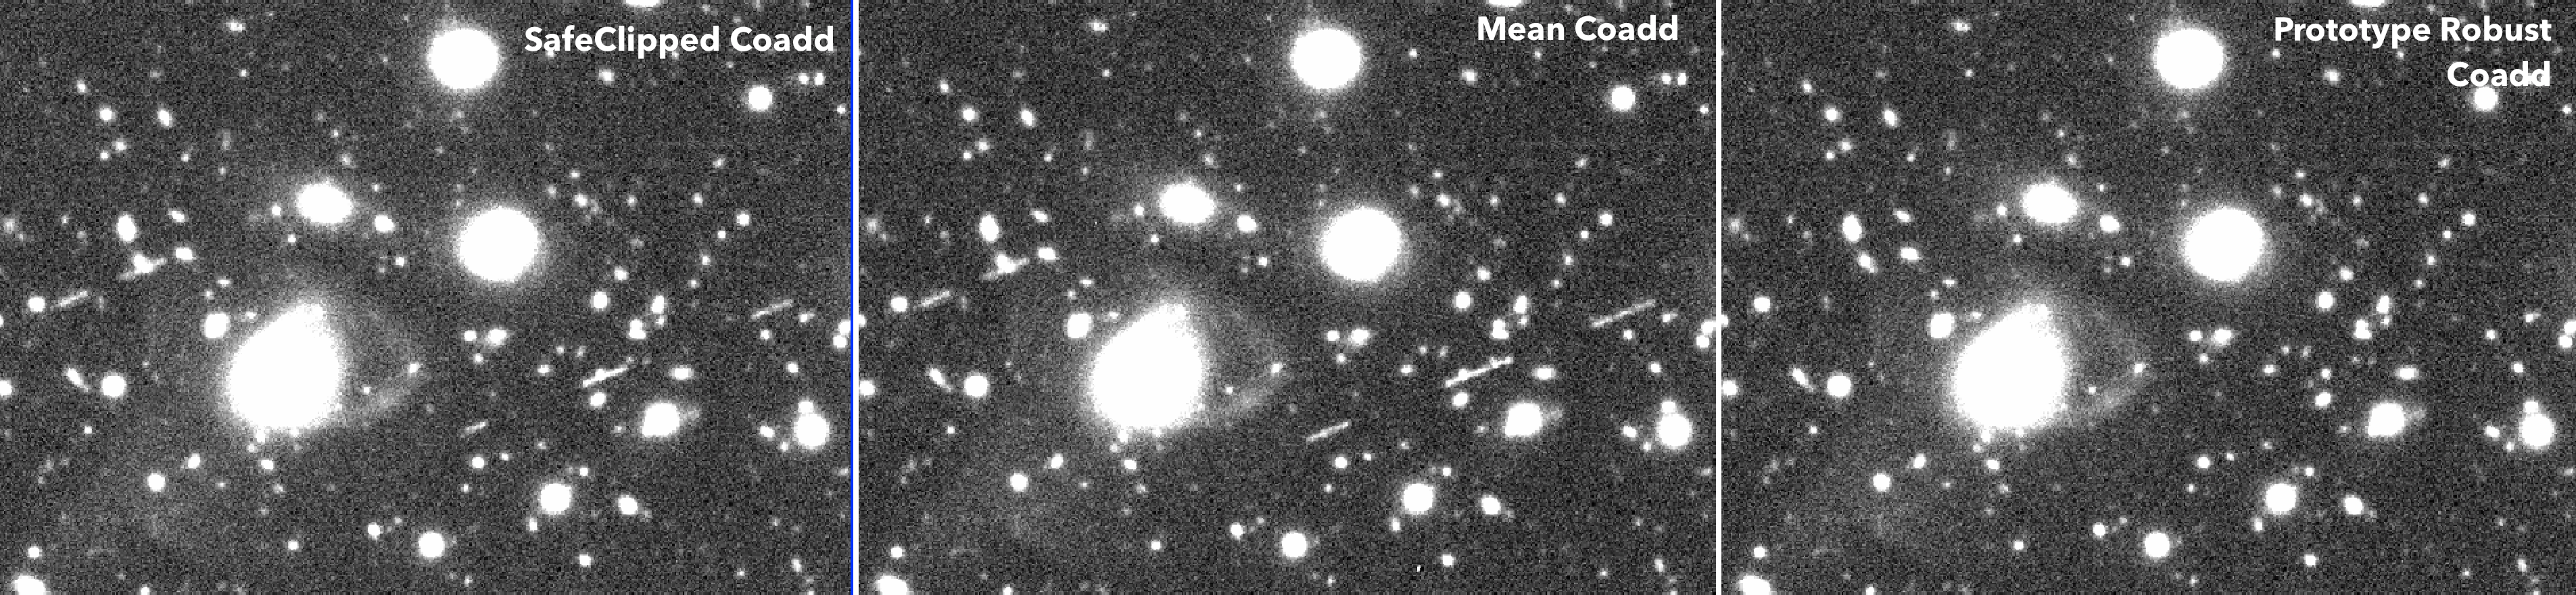
\includegraphics[width=0.5\textwidth]{figures/warpcompare.png}\\
  \tiny Figure: AlSayyad.
  \end{center}
}

\end{frame}


\frame {\frametitle{Alerts }

  \begin{itemize}
  \item \textbf{LDM-503-3: Alert generation milestone}
  \begin{itemize}

    \item First(equal) post-replan milestone  hit by the DM project \citeds{DMTR-53}!
    \item{Demonstrating a \textit{end-to-end} alert production pipeline.}

  \end{itemize}
\item Prototype alert distribution system using Kafka \& AVRO; benchmark results on \citeds{DMTN-028}.
\item   New MOPS (Moving Object)  linking algorithm under development and approach to Minor Planet Center \citeds{DMTN-087}.
  \end{itemize}


  \vspace{-0.5cm}
  \begin{columns}
    \begin{column}{0.72\textwidth}
      \begin{itemize}
	\item Jointcal replaces meas\_mosaic
      \begin{itemize}
        \item{Simultaneous astro- and photometric fitting to source lists derived
        from multiple images.}
        \item{The all new, much improved, more generic replacement for the
        HSC-specific meas\_mosaic.}
      \end{itemize}
      \end{itemize}
\tiny
\vspace{-5pt}
Figure shows the variation in photometric calibration not captured by single frame processing, normalized to 1.
\vspace{-5pt}
This demonstrates fine structure in photometry which Jointcal picks up but per-CCD processing doesn't catch.
\normalsize

    \end{column}

    \begin{column}{0.28\textwidth}
\vspace{-20pt}
      \begin{center}
        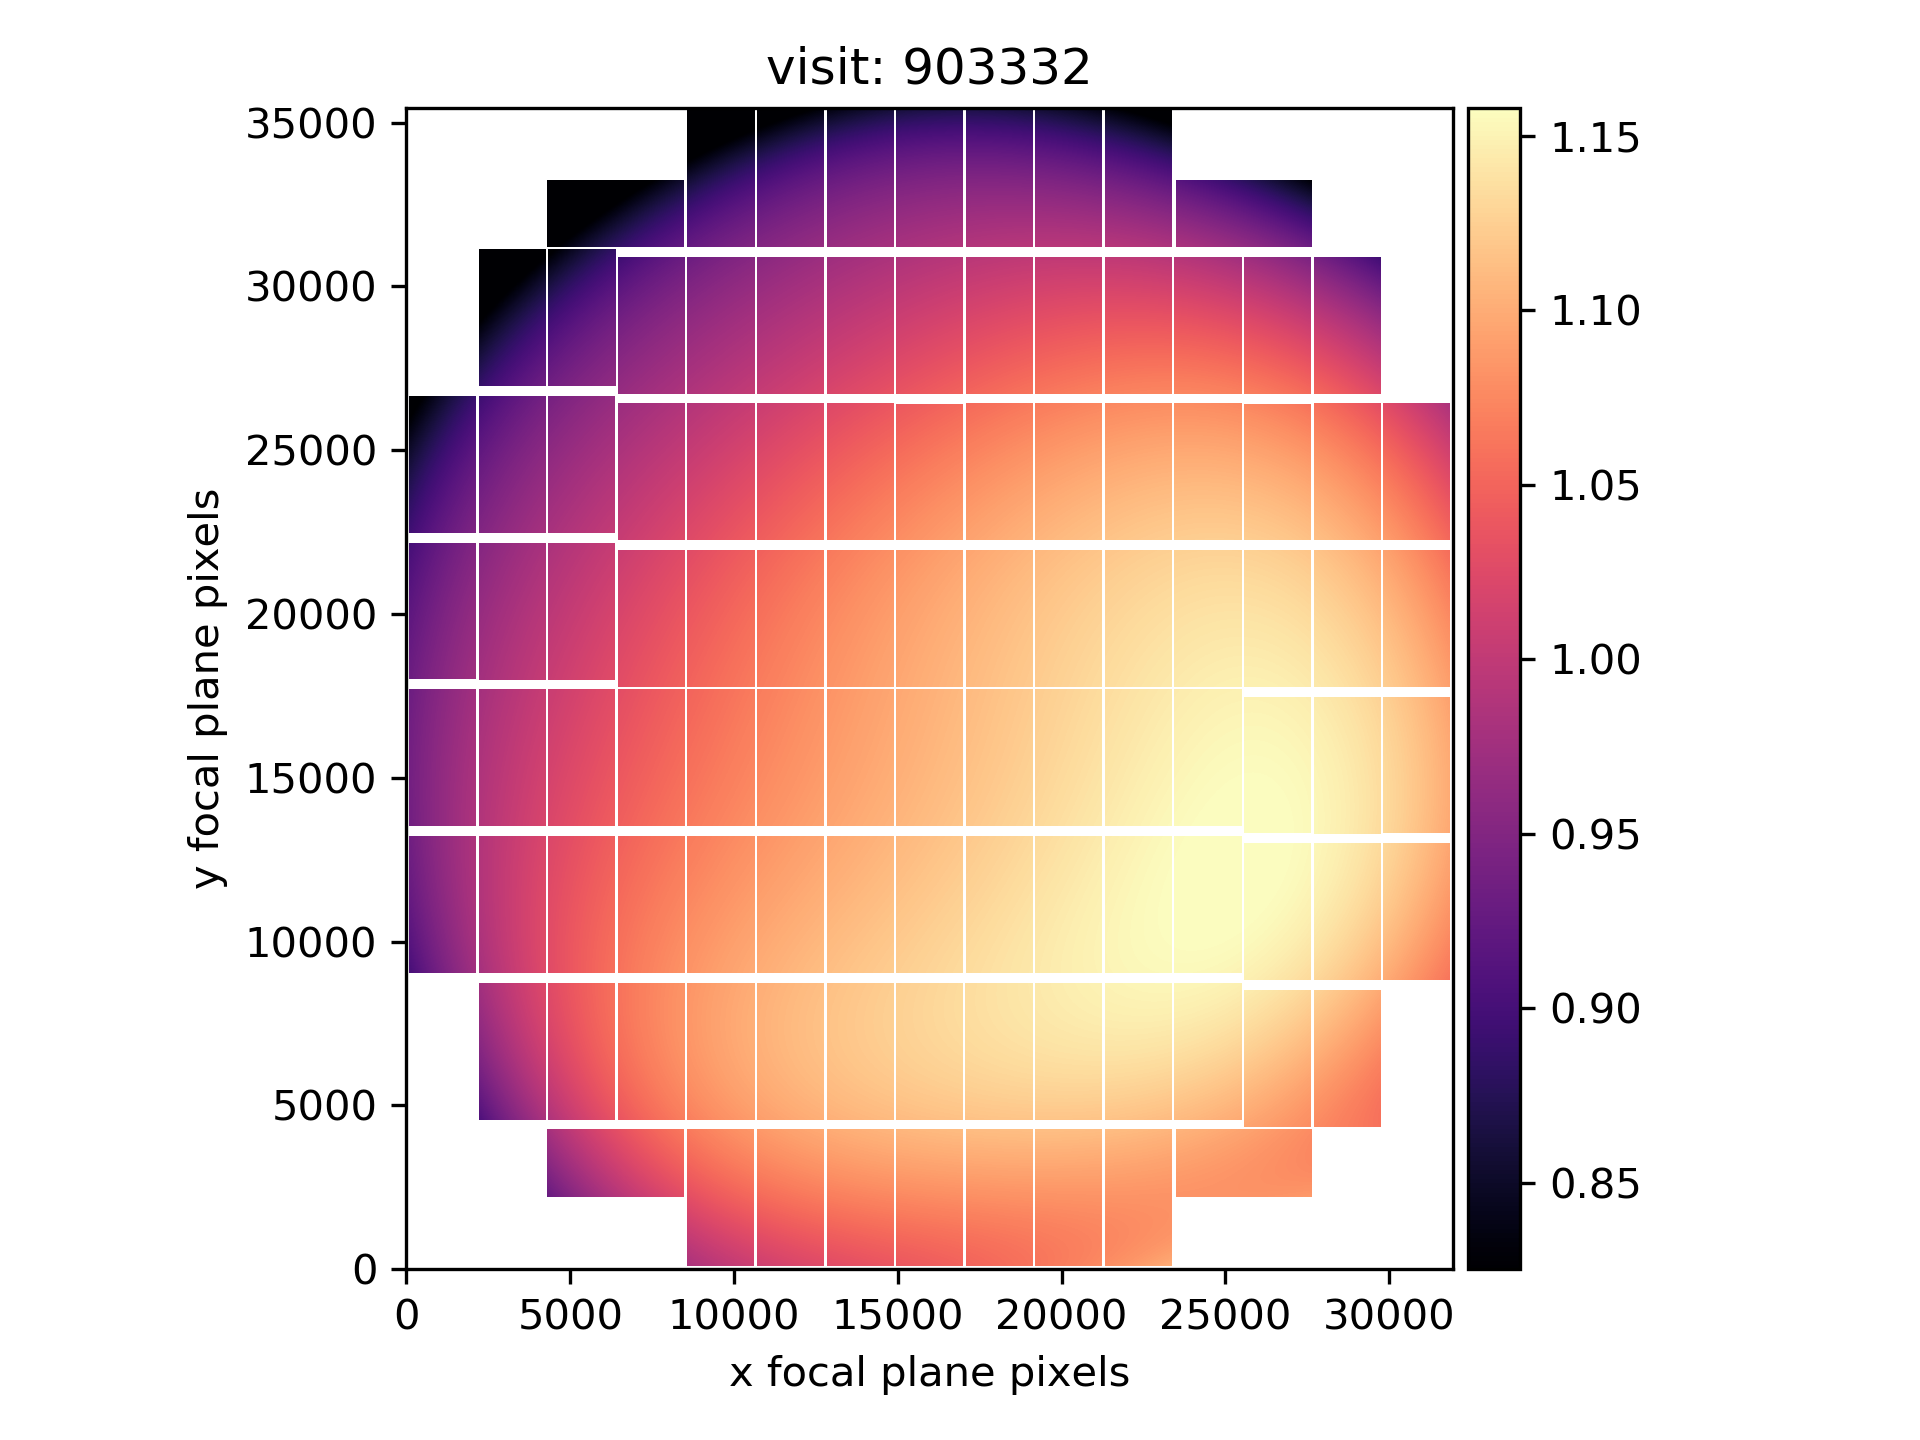
\includegraphics[width=1.0\textwidth]{figures/jointcal.png}\\
        \tiny Figure: Parejko.
      \end{center}
    \end{column}
  \end{columns}

}

\frame{\frametitle{Base \& Network: Fiber First Light }

\begin{columns}
\begin{column}{0.75\textwidth}
Successful transfer of digital data over LSST/AURA fiber optic networks from the Summit Site on Cerro Pachon to NCSA.  A set of 6 x 10 Gbps Network Interface cards on Data Transfer Nodes (DTN) configured with iPerf3 generated a sustained data rate of approximately 44 gigabits per second, over a period of 24 hours, exceeding the target of 40 gigabits per second.

\includegraphics[width=\textwidth]{net_firstlight}\\
\end{column}
\begin{column}{0.25\textwidth}
\vspace{0.3cm}
(\citeds{Document-28547})
\includegraphics[width=\textwidth]{net_firstlight_op}\\
\includegraphics[width=\textwidth]{net_firstlight_screen}
\end{column}
\end{columns}


}


\frame{\frametitle{Data Access Services }
\begin{columns}
    \begin{column}{0.6\textwidth}
        \begin{itemize}
            \item Catalog Database (Qserv) to 100 TB range
            \begin{itemize}
                \item Three 30-node clusters operating:
                \begin{itemize}
                    \item NCSA (PDAC): science dataset (Stripe 82 + AllWISE + NEOWISE)
                    \item CC-IN2P3 (2 x dev): synthetic dataset
                \end{itemize}
                \item 30\% DR1 KPM measurements \citeds{DMTR-17}
                        \item Deployment under Kubernetes
            \end{itemize}
	\item Gen 3 Data Butler and Supertask in progress
        \end{itemize}
    \end{column}
    \begin{column}{0.4\textwidth}
        \begin{center}
            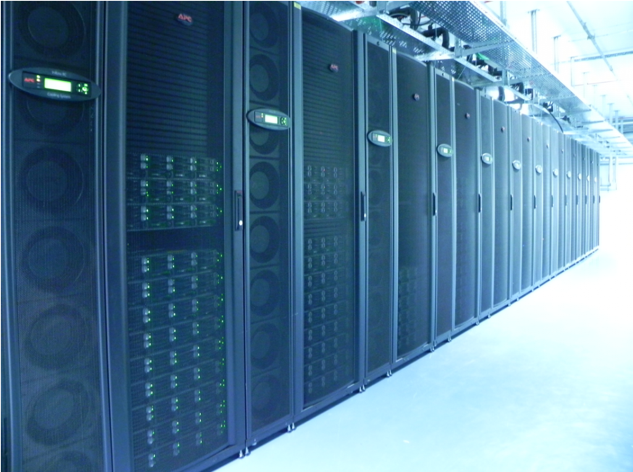
\includegraphics[width=\columnwidth]{figures/qserv-in2p3.png}
	{\tiny \bf IN2P3 Qserv Cluster - Fritz Muller}
        \end{center}
    \end{column}
\end{columns}
}



\frame{\frametitle{LSST Data Facility (NCSA) }
\begin{columns}
\begin{column}{0.5\textwidth}
\vspace{-6.3cm}
\begin{itemize}
\item  Observatory Operations Support (Level 1) Services

\begin{itemize}
\item Working within the LSST Systems Engineering Early Pathfinder group, developing and testing integration of T\&S, Camera, and DM service software via a series of early integration activities.
    \item Initial header service developed and configured for Camera subsystem and AuxTel use cases, ability to acquire pixel data and write FITS files, all commandable by OCS. Demonstrated on Level 1 Test Stand \citedsp{DMTR-61} and with Spectrograph in Tucson

\end{itemize}
\end{itemize}
\end{column}

\begin{column}{0.5\textwidth}
\includegraphics[width=1\textwidth]{EIA-341-Tucson-2018}\\
EIA-341 reading image from the spectrograph in Tucson July 2018
\end{column}
\end{columns}
}

\frame{\frametitle{Science Platform Vision to Reality (1.1) }
%\vspace{-10pt}
\vspace{-5pt}
Vision: \citeds{LSE-319} --- Design: \citeds{LDM-542} --- Test: \citeds{DMTR-51} at NCSA

\begin{columns}
\begin{column}{0.7\textwidth}
\includegraphics[width=1\textwidth]{images/psfnb}
\end{column}
\begin{column}{0.3\textwidth}
\vspace{-7cm}
\\
Portal/Browser\\
Notebooks\\
Web API\\
(Batch)\\
\hspace{-1.5cm} \includegraphics[width=1.3\textwidth]{images/firefly}\\
\hspace{0.1cm} {\tiny \bf Images Krughoff($\leftarrow$) and Wu ($\uparrow$)}
\end{column}
\end{columns}

}
